\subsection{Controlador}
El controlador en un MVC es el responsable de recibir y procesar la entrada del usuario y actualizar el modelo. En esta práctica el controlador es especialmente extenso, pues es responsable de: \begin{itemize}
    \item Detectar si un número es primo.
    \item Identificar los factores de un número.
    \item Generar datos de estimación temporal.
    \item Generar claves RSA de tamaño parametrizado.
    \item Encriptar y desencriptar texto.
    \item Comprimir y descomprimir archivos.
\end{itemize}

\subsubsection{Diseño}
\paragraph{Primalidad}\label{sec:primality}
Para detectar si un número es primo o no, se han desarrollado un conjunto de algoritmos que el usuario, bajo su libre albedrío, puede ejecutar:\\

\begin{itemize}[leftmargin=13pt]
    \item Trial division\cite{Trial division}: Consiste en dividir el número que se quiere comprobar si es primo por todos los números primos menores que su raíz cuadrada. Si el número es divisible por alguno de estos números, entonces no es primo. Si no es divisible por ninguno de ellos, se considera primo.\begin{itemize}
        \item \textbf{Complejidad temporal}: $O(\sqrt{N})$ ya que comprobamos en un bucle por dicha condición.
        \item \textbf{Complejidad espacial}: $O(1)$ al no necesitar ninguna estructura adicional que dependa del tamaño del número.
    \end{itemize}\bigskip

    Adicionalmente, se ha implementado una modificación de dicho algoritmo utilizando \say{thread pools}\cite{Thread pools in Java}, creando así una ejecución paralela del algoritmo.\bigskip
    
    \item Fermat\cite{Fermat primality test}:
    Basado en el teorema de fermat, establece que si un número \textit{p} es primo, entonces para cualquier número entero \textit{q} menor que \textit{p}, se cumple que $q^{p-1}\equiv 1 \texttt{ mod } p$. Matemáticamente:
    \[prime(p) \longleftrightarrow \forall q \mid q < p \implies q^{p-1} \equiv 1 \texttt{ mod } p\]
    Para ello, se escoge un número aleatorio \textit{q} y se verifica dicha congruencia. Como se puede apreciar, el algoritmo es probabilístico, lo que implica que, bajo las peores circunstancias posibles, el algoritmo podría no acabar nunca, además de poder ofrecer falsos positivos. La repetición de este proceso con diferentes valores de \textit{q} aumenta la confianza de dicha congruencia. En nuestro caso, dicho número de iteraciones y semilla para la generación de valores aleatorios está parametrizada, por lo que los resultados se pueden replicar nativamente.
    \begin{itemize}
        \item \textbf{Complejidad temporal}: Impredecible al ser un algoritmo probabilístico.
        \item \textbf{Complejidad espacial}: $O(1)$ al no necesitar ninguna estructura adicional que dependa del tamaño del número.
    \end{itemize}\bigskip
    
    \item Miller Rabin\cite{Miller–Rabin primality test}:
    Basado en el teorema de Miller Rabin, establece que si un número compuesto \textit{n} pasa ciertas pruebas de primalidad entonces es probable que sea primo. Por cada iteración del algoritmo, es escoge un valor aleatorio \textit{q} y se verifica si cumpla dicha condición. Si no la cumple se le denota como compuesto, mientras que si la cumple para todas las otras, incluida la misma, se le denota como posible primo. Al igual que en el algoritmo de Fermat, la confianza es directamente proporcional a la cantidad de iteraciones usadas.
    \begin{itemize}
        \item \textbf{Complejidad temporal}: Impredecible al ser un algoritmo probabilístico.
        \item \textbf{Complejidad espacial}: $O(1)$ al no necesitar ninguna estructura adicional que dependa del tamaño del número.
    \end{itemize}\bigskip

    Adicionalmente, se ha implementado una modificación de dicho algoritmo utilizando \say{thread pools}\cite{Thread pools in Java}, creando así una ejecución paralela del algoritmo.\bigskip
\end{itemize}\bigskip

\paragraph{Identificación de factores}
Para identificar los factores de un número arbitrariamente grande se ha desarrollado el siguiente algoritmo, cuyo pseudocódigo podría ser el siguiente: \begin{code}{\scriptsize}{python}
def get_factors(num):
    prime_factors = {}
    divisor = 2

    while num > 1:
        if num.isPrime():
            prime_factors[num] = 1
            break

        if num % divisor != 0:
            divisor = divisor.nextPrime()
            continue

        prime_factors[divisor] = prime_factors.get(divisor, 0) + 1
        num = num // divisor

    return prime_factors
\end{code}

El algoritmo usa una \texttt{Map} donde sus claves vienen determinadas por los diferentes números primos que encontremos y su valor es su frecuencia; creando así un mapa de frecuencias. El caso base, definido en la línea 6, determina si el elemento ya es primo y, por ende, no existirán más factores además de él. Si no es el caso, revisamos si es divisible por el actual divisor (inicializado a 2) si no lo es, cogemos el siguiente valor primo y reiteramos el bucle. En el caso de que si sea divisible, hemos encontrado un factor, por lo que lo añadimos al mapa de frecuencias y modificamos el valor de nuestro número. Al final, después de todo este proceso, retornamos dicho mapa.\bigskip

La complejidad temporal de dicho algoritmo depende de varios factores:\begin{itemize}[leftmargin=13pt]
    \item Implementación de los métodos \texttt{isPrime} y \texttt{nextPrime} que, al estar dentro de un bucle, podrían afectar gravemente al rendimiento de la aplicación.
    \item La búsqueda de factores primos como tal que, en el peor de los casos y para un número no primo, se ejecutará hasta que dicho se reduzca a 1. En general, podemos asumir que el número de iteraciones depende de la cantidad de factores primos que tenga dicho número y por ende será proporcional al dicho.
\end{itemize}
Así pues, la complejidad temporal asintótica de este método se podría expresar como $O(K * F)$ donde \textit{K} es el coste de implementación de los previos métodos y \textit{F} la cantidad de factores que tiene un número.\bigskip

Espacialmente, al estar generando un mapa de frecuencias, se toma como $O(F)$ donde \textit{F} es la cantidad de factores para un número arbitrario, al tener que crear una entrada en el mapa por cada factor diferente.\bigskip

\paragraph{Generación de datos temporales}
Para evitar esperas significativamente altas a la hora de identificar los factores de un número arbitrario, se ha implementado un breve estudio que permite estimar su tiempo de ejecución. Comentar que, debido al uso de una \href{https://en.wikipedia.org/wiki/Newton_polynomial}{interpolación polinómica de newton} dicha estimación depende del hardware en el que se ejecute el muestreo de datos y, por ende, no será preciso en otras máquinas. Para ello se usó \href{https://planetcalc.com/9023/?xy=5%2010%0A7%2023%0A8%2061%0A10%20165%0A11%20428%0A14%2016596%0A15%2037864&interpolate=10%2020%2030%2040}{planetcalc} que permite, identificando un conjunto de puntos, efectuar dicha interpolación. Así pues podemos obtener el siguiente resultado:
\begin{figure}[!h]
    \centering
    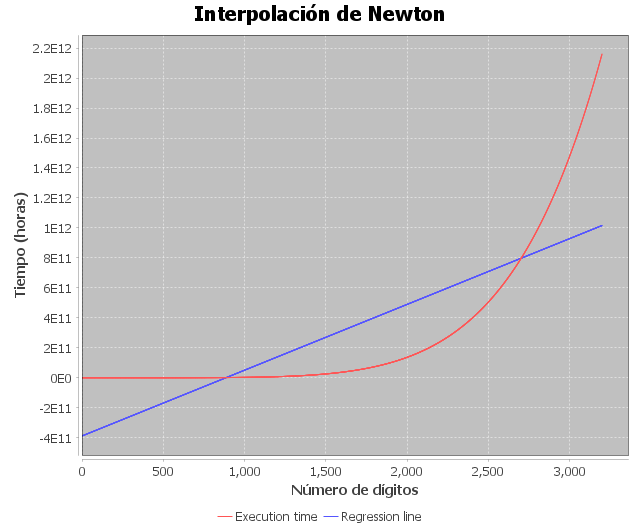
\includegraphics[width=\linewidth]{MVC/Controller/img/newton interpolation.png}
    \caption{Interpolación de newton}
    \label{fig:newtoninterpolation}
\end{figure}

Como se puede apreciar, podemos ver la propia función en \textcolor{red}{rojo} y la regresión lineal en \textcolor{blue}{azul}. Con respecto a su forma, aun sabiendo que es una polinómica de sexto grado, se podría decir que, bajo el dominio $[0, \infty)$ presenta una curva exponencial. Así pues, la función que devuelve los factores de un número dado primero evalúa si, con respecto a esta función, dicha ejecución tardaría más que cierto límite (en nuestro caso, un minuto); Si es así, no se calcula y se le informa al usuario cuanto tiempo aproximadamente tardaría dicho cálculo.\bigskip

\paragraph{Generación de claves RSA}
Para dicha generación se han implementado dos métodos. El primero genera un número primo de \textit{X} cifras, usado para poder determinar \textit{aproximadamente} el tamaño de la clave RSA. Esto se debe a que, para crear dicha clave, se generaran dos números de longitud \textit{X} que se usarán como los parámetros \textit{p} y \textit{q}. Ya que los multiplicamos para determinar \textit{n}, y bajo aproximación, determinamos que la longitud de un número \textit{A} sigue el siguiente teorema:
\[\forall A, A = B \cdot C  \implies \mid A \mid  = \mid B\mid + \mid C\mid\]

Así pues, y mediante una implementación probabilística, generamos números de \textit{X} cantidad de valores e identificamos si es primo; en tal caso lo devolvemos.\bigskip

El segundo algoritmo genera la propia pareja de claves RSA, cuyo pseudocódigo, podría ser el siguiente:
\begin{code}{\scriptsize}{python}
def generate_key_pair(p, q, seed):
    n = p * q
    
    phi = (p - 1) * (q - 1)
    
    rng = random(seed)
    
    e = None
    while True:
        e = rng.randint(1, phi - 1)
        if gcd(e, phi) == 1:
            break
    
    d = powmod(e, -1, phi)
    
    return KeyPair(
        PrivateKey(d, n),
        PublicKey(e, n)
    )
\end{code}

Donde se efectúan los siguientes pasos: \begin{enumerate}
    \item Se genera \textit{n} como el producto de \textit{p} y \textit{q}.
    \item Se obtiene $\phi(n)$ como $(p-1)\cdot(q-1)$.
    \item Se calcula \textit{e} tal que $0 < e < \phi(n)$ y tanto \textit{e} como $\phi(n)$ son coprimos mediante un bucle.
    \item Se calcula \textit{d} como el inverso multiplicativo modular\cite{Modular multiplicative inverse} de $e \texttt{ mod } \phi(n)$.
    \item Finalmente, se retorna la pareja de claves RSA
\end{enumerate}\bigskip

\paragraph{Encriptación}
Una pareja de claves RSA contiene un conjunto de métodos que permiten encriptar y desencriptar tanto texto como ficheros. Ambos utilizan un metodo de exponenciación modular\cite{Modular exponentiation} cuya implementación sigue el siguiente pseudocódigo:
\begin{code}{\scriptsize}{python}
def modular_exponentiation(base, exponent, modulus):
    result = 1

    while exponent > 0:
        if exponent & 1:
            result = (result * base) % modulus
        base = (base * base) % modulus
        exponent >>= 1

    return result
\end{code}
Esencialmente, solo podemos encriptar (y por ende desencriptar) números; por ello, en el caso de querer encriptar un texto, debemos iterar por todos sus caracteres, convertirlos en sus valores ASCII y encriptar dicho valor; lo que se podría implementar de la siguiente manera:
\begin{code}{\scriptsize}{java}
for (String string : text.split("\n")) {
    string.chars().forEach(e -> 
        encryptedText
            .append(
                publicKey
                    .encrypt(String.valueOf(e))
                    .toString()
            )
            .append("\n");
	);
	// Add special character to indicate EOL 
	encryptedText.append("@\n");
}
\end{code}
Como se puede apreciar, iteramos por todas las líneas y por cada valor ASCII los encriptamos y añadimos al string encriptado. Adicionalmente, se puede ver como añadimos un terminal \say{@} al final de cada línea tratada. Esto nos permite fácilmente reconvertir el texto completo, ya que transformar el final de la línea en Linux y Windows nos daba ligeros problemas de inconsistencia.\\

El proceso de des encriptación sigue la misma estructura, desencriptando cada línea a un carácter y transformando el terminal en un salto de línea, como se puede ver aquí:
\begin{code}{\scriptsize}{java}
for (String string : text.split("\n")) {
	if (string.equals("@")) {
		decryptedText.append("\n");
		continue;
	}
 
	decryptedText
        .append((char) privateKey
            .decrypt(string)
            .intValue()
        );
}
\end{code}
\paragraph{Compresión}
Para este proyecto se ha añadido la posibilidad de guardar un archivo encriptado o desencriptado a disco. Adicionalmente, y para reducir el tamaño de dichos archivos, se ha decidido comprimirlos mediante el formato de compresión \href{https://en.wikipedia.org/wiki/ZIP_(file_format)}{ZIP}, usando \texttt{Deflater} y \texttt{Inflater} que permiten, respectivamente, comprimir y descomprimir \say{streams} de datos. Esto nos permite, de media, reducir hasta cinco veces el tamaño de los archivos guardados. Además de ello, la aplicación puede leer archivos tanto encriptados como no encriptados, debido al uso de una extensión especifica que se fuerza a la hora de guardar un archivo desde la aplicación. 

\subsubsection{Estudios}\label{sec:algt_studies}
    
\paragraph{Detección números primos}\label{Prime study}

 Para el estudio del rendimiento de los algoritmos, se ha realizado una serie de tests. Estos tests consisten en la ejecución de los algoritmos, concretamente, 10000 veces para un determinado número primo de 1683 dígitos. A partir de los datos obtenidos se han guardado en una base de datos para poder analizar los datos con \say{Jupyter Notebooks} para obtener una mayor facilidad y versatilidad del análisis de los datos. En estos \say{notebooks}, se analizan profundamente los resultados obtenidos de los tests, específicamente, se analiza la estabilidad y el rendimiento en tiempo de ejecución de estos algoritmos.\\

 A partir del análisis realizado, se obtiene la conclusión de que los datos obtenidos son similares entre ellos, aun así se pueden diferenciar con claridad entre ellos. Además, se puede observar cuanto de estables con los algoritmos, el más estable es el que tiene menos anomalías en los datos, es decir, el que tiene menos picos y valles, en este caso, el \say{millerRabin} en paralelo y el menos estable, en este, el \say{miller Rabin} iterativo. Aun así, que sea más estable no significa que sea más eficiente, ya que puede ser más estable pero tardar más en ejecutarse y viceversa, ya que, el que tiene de media un menor tiempo de ejecución es la división iterativa en paralelo del número primo y el más lento de media la división iterativa del número primo.\\
 
Por lo que, a la hora de elegir un algoritmo se debe tener en cuenta tanto su estabilidad como su eficiencia.\\
 
\paragraph{Factorización números}\label{Factor study}

Para el estudio del rendimiento de los algoritmos, se ha empleado una estimación de lo que se tardaría en obtener los factores del número, ya que la factorización de un número es muy costosa. Concretamente, se ha empleado la interpolación de newton, donde la entrada es el número de cifras y la salida el tiempo estimado en horas. A partir de los datos obtenidos se han guardado en una base de datos para poder analizar los datos con \say{Jupyter Notebooks} para obtener una mayor facilidad y versatilidad del análisis de los datos, al igual que en el anterior estudio.\\

En este estudio, únicamente, se visualiza la estimación del coste junto a su regresión lineal para apreciar el coste de factorizar un número.\\

Para ver con más detalle como se han analizado los datos y los resultados, de los apartados \ref{Prime study} y \ref{Factor study}, se pueden encontrar en los PDF adjuntos y en la carpeta \say{tools}. En el directorio \say{tools} contiene el código fuente de los tests y los \say{Jupyter notebooks}.
